\chapter{NAO}\label{NAO}

\section{Vorüberlegungen}
Aus dem Szenario des Gesamtprojekts gingen bei unseren Vorüberlegungen zwei Hauptaufgaben für das NAO Team hervor. Zum einen ist das die Kalibrierung der NXT-Roboter während der Erkundungsphase auf unbekanntem Gebiet. Und zum anderen muss die Zielfindung des humanoiden NAO-Roboters, nachdem das Gebiet erkundet und eine konkrete Route zum Hotspot gefunden wurde, eingeleitet werden.
Unter der Kalibierung der NXT Roboters soll verstanden sein, dass der NAO Roboter mit Hilfe seiner Sensoren den NXT lokalisieren und diese berechnete Entfernung dem MCC mitteilen soll. Eine Kalibrierungsanfrage erfolgt immer nur aus Richtung des MCC an den NAO und zwar dann, wenn ein NXT ``verloren gegangen ist'', d.h. dieser keine genauen Daten mehr liefert.
Zunächst einmal bietet der Hersteller Aldebaran auf seiner Website%
	\footnote{http://www.aldebaran-robotics.com/documentation/index.html} eine recht umfangreiche Dokumentation. Diese ist, wie wir nach längerer Zeit aber feststellen mussten teilweise sehr schlecht. Es ist oft nicht klar, was die Daten, die man z.B. über die Sensoren abgreifen kann tatsächlich bedeuten. Dieses Problem trat beispielsweise bei den NAOMarks oder bei dem Sonar auf. In dem Abschnitt Probleme und Lösungen wird darauf noch eingegangen werden.
Gemeinsam mit den anderen Teams überlegten wir uns als einheitliche Programmiersprache Python zu verwenden, da sie sowohl von dem NXT-Mindstorm Robotern, als auch vom NAO unterstützt werden. Es hat sich allerdings herausgestellt das für die Programmiersprache C++ deutlich mehr Beispiele auf der Aldbaran Webseite vorliegen und die Dokumentation dafür besser ausgeführt ist.
Bei Aldebaran gibt es eine API, die es erlaubt vordefinierte Schnittstellen z.B. der Sensoren des NAOs zu benutzen.

\section{Software NAO}
\subsection{NAOqi}
NAOqi ist ein Framework von Aldebaran, was auf dem NAO läuft und den Roboter steuert. Es ist hardware- und plattformunabhängig. Für verschiedene Programmiersprachen wie z.B. C++ oder Python stellt Aldebaran ein Software Development Kit (SDK for NAOqi) bereit, um das Implementieren von Programmen auf dem NAO in verschiedenen Sprachen möglich zu machen.
Jede Maschine, auf der die NAOqi läuft, erschafft einen Broker. Jeder Broker verwaltet die Module, die innerhalb von ihm ausgeführt werden. Wenn ein Modul aufgebaut ist, bekommt es einen Zeiger auf den Broker übergeben. Module können Funktionen der anderen Module durch einen Proxy, der durch den Broker erzeugte wird, aufrufen.
Der Broker abstrahiert die Netzwerk-Schnittstelle auf den Maschinen, so dass, wenn eine Funktion über einen Proxy aufgerufen wird, diese Funktion möglicherweise auf einer anderen Maschine im Netzwerk ausgeführt werden kann.
\\
\begin{figure}[ht]
    \centering
	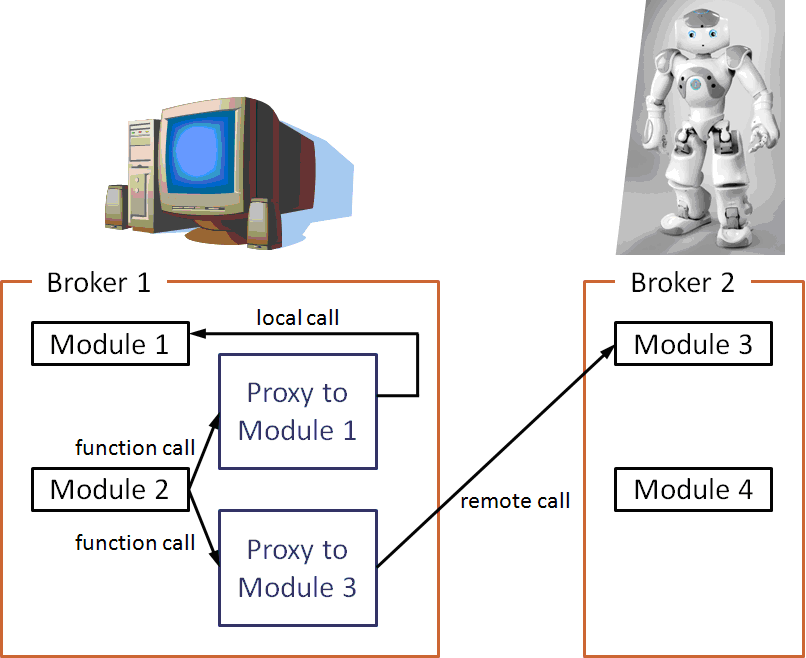
\includegraphics[width=0.7\textwidth, angle=0]{img/nao_1.png} 
\end{figure}
Innerhalb des NAOqi Prozesses laufen verschiedene Module. Wir verwenden diese Module:
\begin{enumerate}
\item ALLandMarkDetection: wird verwendet, um NAOMarks zu finden und zu erkennen
\item ALMemory: zum erignisbasierten Speichern von Daten
\item ALMotion: ansprechen der Motoren zum Bewegen des NAO
\item ALVideoDevice: erlaubt Zugriff auf die beiden Kameras des NAO
\end{enumerate}

\subsection{Choreographe}
Choreographe ist ein graphisches Programmierinterface. Durch das Auswählen und Verbinden von vorgefertigten Funktionsboxen kann man schnell und intuitiv erste Programme erzeugen und direkt auf dem NAO oder mit der Software NAOsim testen.
Alle Hauptfunktionen des NAOs wie beispielsweise die Steuerung aller Gelenke können mit verschiedensten Konfigurationen getestet werden. Dadurch ist dem Benutzer schnell ermöglicht erste Erfahrung mit dem Umgang des Roboters zu gesammelt. Wenn eine Verbindung zu einem NAO vorhanden ist, kann über ein dreidimensionales Robotermodell jeder Motor einzeln angesprochen werden. Darüber hinaus kann in einem weiteren Fenster das aktuelle Kamerabild angezeigt werden.
\subsection{Weitere Software}
\subsection*{NAOsim}
NAOsim ist ein Simulationsprogramm, womit ein vollständiger NAO simuliert werdern kann. Es ist möglich Testumgebungen selbst zu erschaffen, indem mach sich beispielsweise einen Raum mit Hindernissen einrichtet. Dadurch sind auch Tests einen realen NAO möglich. Auf einen realen Test sollte man allerdings keinesfalls verzichten, da NAOsim immer vollständig exakte Werte und Bewegungen des NAOs simuliert.
\subsection*{Monitor}
Dies ist ein Programm, dass das aktuelle Kamerabild oder alternativ die Sensordaten des NAOs auslesen und aufzeichnen kann. Das Programm ist vor allem dann hilfreich, wenn mit der Detektion von NAOMarkern gearbeitet wird. Es ist möglich über Monitor einzelne Einstellungen der Kamera wie beispielsweise Helligkeit, Kontrast, Gain, Auflösung, Sättigung oder Farbton vorzunehmen. 

\section{Hardware NAO}
In unseren Tests und für das Szenario selbst benutzen wir einen NAO H21 Body. Dieser zeichnet sich durch verschiedenste Sensoren aus. Es sind zwei Infrarotsensoren, drei Trägheitsmesser (2x Schwingungs- und 1x Beschleunigungssesoren), Kontaktsensoren für Brust, Füße und Kopf, Sonar (2 Empfänger und 2 Sender), 32 Positionssensoren, ein Force Sensing Resistor und vier Mikrofone, zwei Kameras, sowie zwei Lautsprecher eingebaut. Das vollständige Datenblatt kann man online bei Aldebaran anschauen%
	\footnote{http://www.technik-lpe.eu/fileadmin/bilder/produkte/aldebaran/NAO\_H21\_Next\_Gen.pdf}.

\section{Messungen}
Wie in dem Abschnitt Sensoren bereits beschrieben wurde, besitzt der NAO Roboter einige Sensoren, die wir vor der Benutzung auf die Genauigkeit verifiziert haben.
Wir haben Messreihen angelegt für die Vorwärtsbewegung des NAOs, also dem einfachen Laufen für das in dem Roboter integrierte Sonar und haben die Kamera auf Schärfe und Brauchbarkeit untersucht.

\subsection{Kamera}
Eine Herausforderung bei dem NAO stellt die integrierte Kamera dar. Da die Kommunikation drahtlos über ein WLan-Netzwerk sehr viel besser funktioniert, als mit Kabel, ist nur eine geringe Auflösung des Kamerabildes möglich (VGA). Alternativ kann auch eine höhere Auflösung (1280x960 Pixel) genutzt werden, dazu muss man aber gleichzeitig eine teilweise stark reduzierte Framerate (1 fps) in Kauf nehmen.
Zusammen mit der Kamera werden wichtige integrierte Funktionalitäten, wie die Erkennung von NAOMarkern und einem Roten Ball (mit genau definierter Größe), mitgeliefert. Diese werden in den nächsten Abschnitten genauer erklärt.

\subsection{Sonar}
Das Sonar des Roboters lässt sich relativ einfach über das bereits vorhandene Beispiel auf der Aldebaran Website%
	\footnote{http://www.aldebaran-robotics.com/documentation/\_downloads/sensors\_sonar.py} auslesen. Dabei gibt es zwei Sonarsensoren im NAO je einen für links und rechts. Die Ergebnisse können in dem hier vorliegenden Diagramm abgelesen werden. Wir habe für jeden Abstand zwischen 2.0 m und 0.1 m, die in 0.1 m Schritten weiter unterteilt sind, jeweils 10 Messungen entnommen und gemittelt. 
Es ist auffällig, aber nicht weiter verwunderlich, dass beim linken Sonar unseres NAOs die Genauigkeit abnimmt, je weiter er sich vom Hindernis entfernt. Beim rechten Sonar dagegen ist die Genauigkeit überraschenderweise auch bei einer Entferung von 1,5 m und größer weiterhin sehr gering (Abweichung < 1 cm). Sowohl bei dem linken, als auch dem rechten Sonar wird die Genauigkeit bei einer geringen Entfernung (<20 cm) gleichermaßen schlechter. 
Bei unseren Messungen haben wir keine Differenzierung in der Oberflächenbeschaffenheit unternommen, sodass unsere Messungen ausschließlich mit einer weißen glatten Wand als Hindernis durchgeführt wurden. Aussagen über andere Oberflächen können daher nicht gemacht werden.

\begin{figure}[ht]
    \centering
	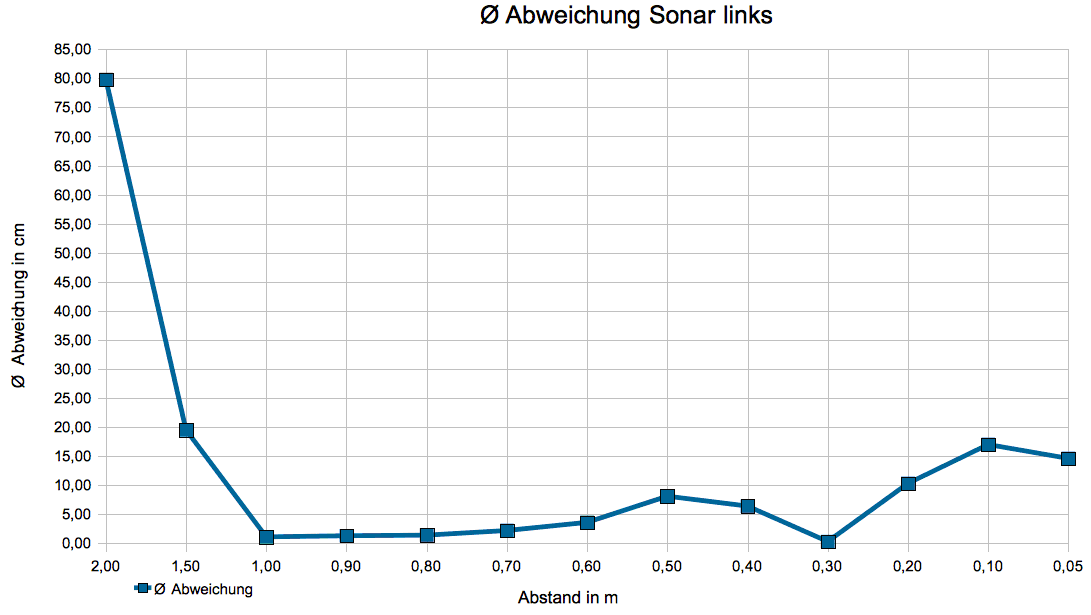
\includegraphics[width=0.9\textwidth, angle=0]{img/nao_2.png} 
\end{figure}

\begin{figure}[ht]
    \centering
	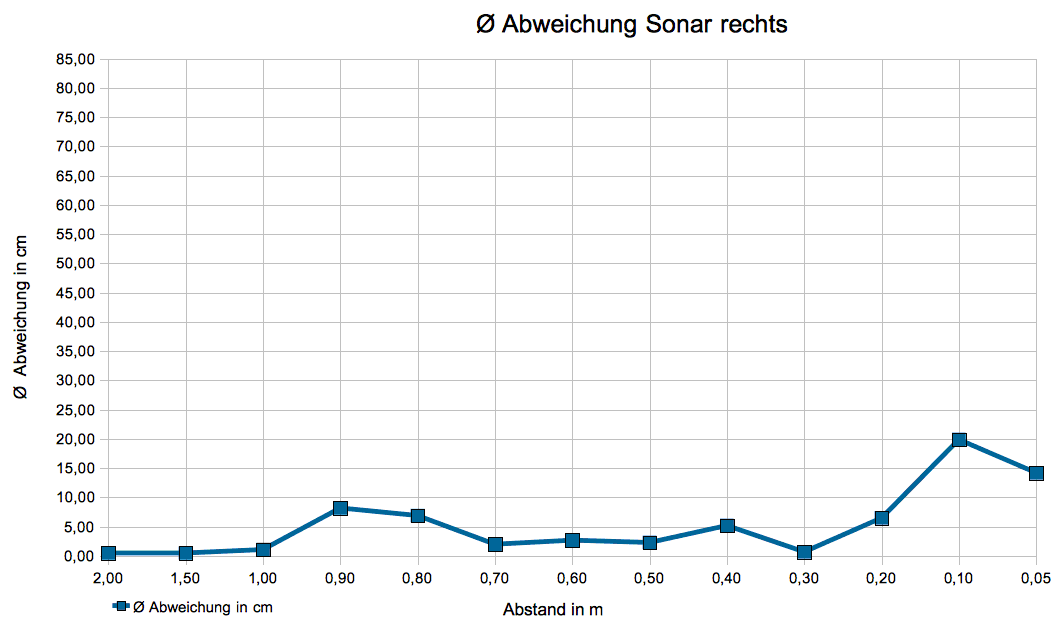
\includegraphics[width=0.9\textwidth, angle=0]{img/nao_3.png} 
\end{figure}

\subsection{NAO Walk}
Für das Szenario unseres Semesterprojektes benötigen wir einen Roboter, der möglichst ohne Abweichungen laufen kann, um sein Ziel zu erreichen.
Man könnte auch annehmen, dass der NAO Roboter sich auf etwas größere Entfernungen trotzdem noch geradlinig bewegt. Dies ist tatsächlich aber nicht der Fall, da unser NAO schon bei kleineren Entfernungen einen deutlichen Drift nach rechts hatte. Um eine konkrete Aussage über die Genauigkeit des Laufens des NAOs treffen zu können und der Abweichung ggf. entgegenzuwirken, haben wir verschiedene Messreihen angelegt. Der NAO bietet über die bereits beschriebene mitgelieferte Software Choreographe die Möglichkeit verschiedenste Einstellungen der Laufbewegung einzustellen, was man natürlich auch über das NAOqi selbst implementieren kann. Einstellbare Parameter für den NAO Walk sind intuitiverweise die X- und Y-Bewegung, in der sich die Laufbewegung vorwärts (X positiv), rückwärts (X negativ), links (Y positiv) und rechts (Y negativ) wiederfinden lassen. Desweiteren gibt es den Parameter Theta, mit der man die Rotation des NAO definieren kann, wobei der Bereich [-1.0, 1.0] eingehalten werden muss und das Minimum (-1.0) die maximale Rotation im Uhrzeigersinn und das Maximum (1.0) die maximale Rotation gegen den Uhrzeigersinn widerspiegelt. Eine weiterere wichtige Einstellung, die man für das Laufen konfigurieren kann, ist die Schrittgröße sowohl für die X- (angegeben als ``MaxStepX''), als auch für die Y-Laufrichtung ``MaxStepY''). Dieser Wert liegt im Bereich von [0.1 cm; 6 cm].
Um zu erkennen welchen Einfluss die Schrittweite auf die Genauigkeit des Laufens an sich hat, haben wir jeweils 6 verschiedene Schrittweiten von 1 cm bis 6 cm in jeweils Zentimeterschritten genommen: Schrittweite\_i = 1 + i [cm] mit i = {0, 1, 2, 3, 4, 5}. Für jede Schrittweite wurden 5 Messungen vorgenommen und die Gesamtstrecke belief silch einmal auf 1 m und zum anderen auf 0.5 m, sodass insgesamt 60 Messungen vorgenommen wurden. Die Ergebnisse sind hier einmal in Tabellenform und einmal als Diagramm deutlich gemacht.
Zum Verständnis der Messergebnisse ist hier auch der Versuchsaufbau schematisch dargestellt.

\begin{figure}[ht]
    \centering
  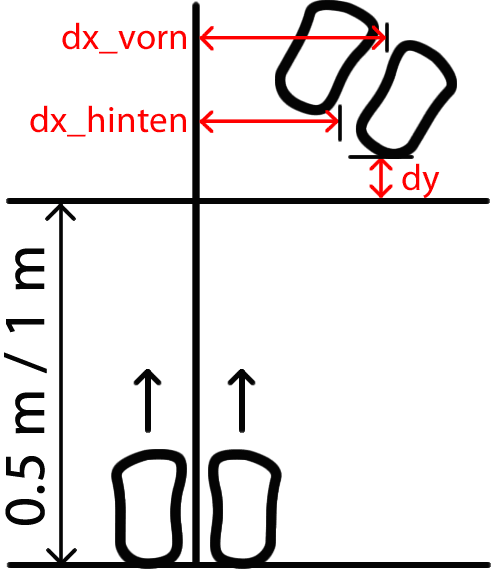
\includegraphics[width=0.5\textwidth, angle=0]{img/nao_4.png}
    \caption{Der NAO läuft 0.5 bzw. 1 m; dx\_vorn und dx\_hinten sind die Abweichungen ausgehend von der Mittellinie zwischen den vorderen bzw. hinteren Füßen (ist der Wert positiv, dann gibt es ein Abdriften nach rechts, andernfalls links); dy gibt an, wie weit der NAO über das Ziel hinausgelaufen ist (ist der Wert positiv, dann ist er zu weit gelaufen, andernfalls zu wenig)}
    \label{nao_foot}
\end{figure}

\begin{figure}[ht]
    \centering
  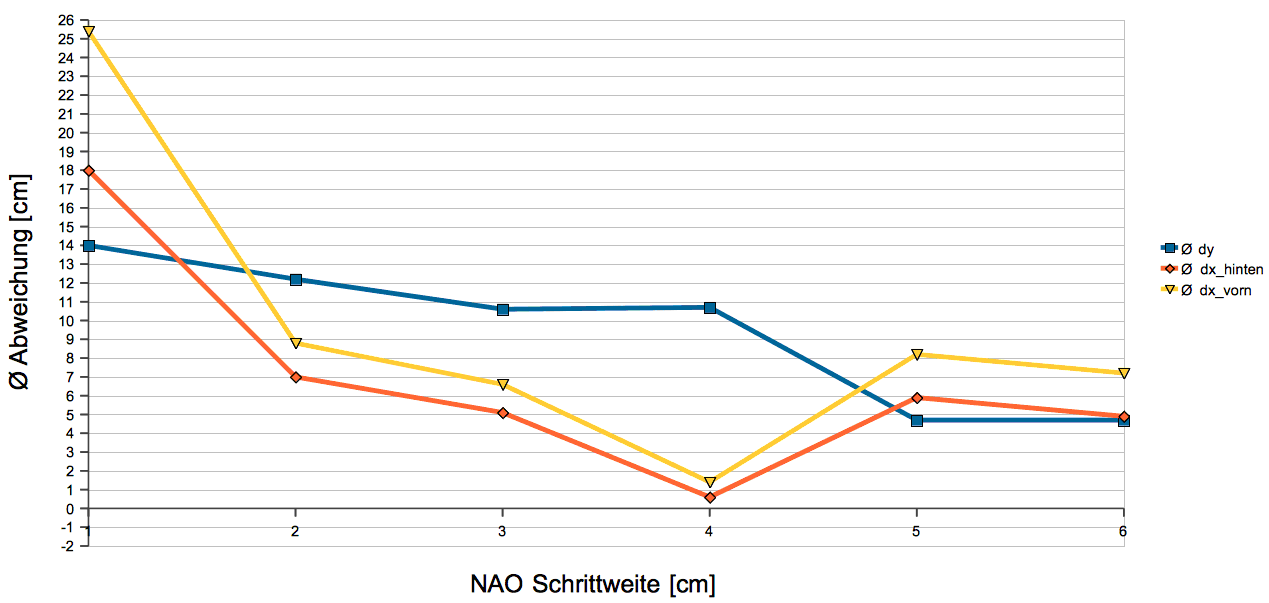
\includegraphics[width=0.9\textwidth, angle=0]{img/nao_5.png}
    \caption{Abweichungen bei 0.5 m Entferung}
    \label{naotab3}
\end{figure}

\begin{figure}[ht]
    \centering
  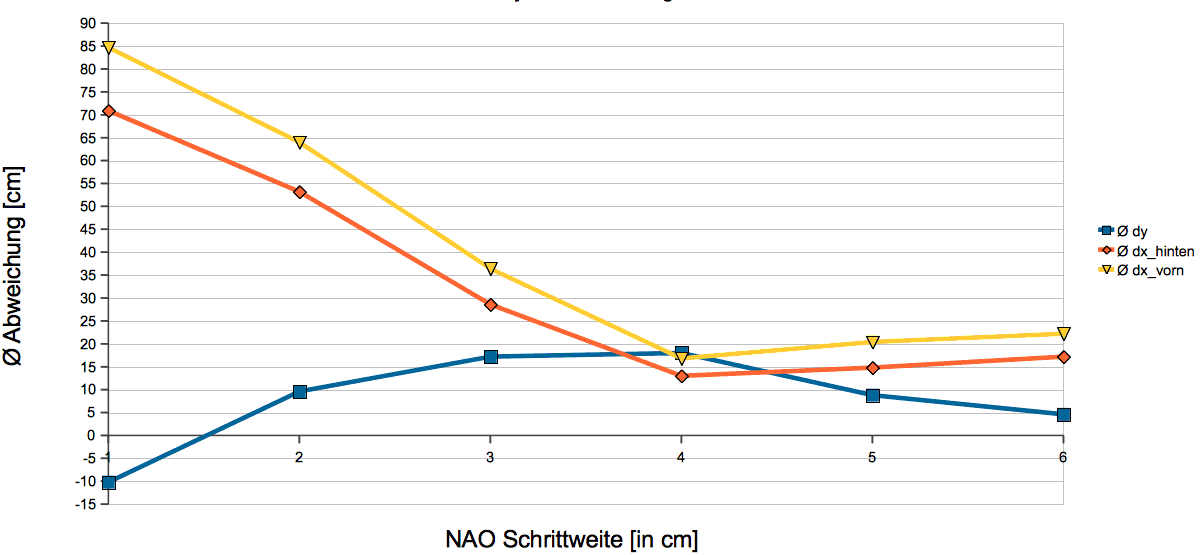
\includegraphics[width=0.9\textwidth, angle=0]{img/nao_6.png}
    \caption{Abweichung bei 1 m Entfernung}
    \label{naotab4}
\end{figure}

\subsection{Auswertung}
Die Visualisierung des Diagramms macht bei beiden Entfernungen (0.5 m und 1 m) deutlich, dass je kleiner die Schrittweite des NAOs ist, die Abweichungen vom Ziel drastisch erhöhen. Daraus lässt sich schließen, dass beim Laufen eine möglichst hohe Schrittweite (Maximum von 6 cm) genommen werden sollte.
Außderdem wird deutlich, dass der NAO fast immer über sein Ziel hinausläuft (dy ist größer 0). 

\subsection{Fazit}
Die Messwerte für den NAO Walk sind scheinbar stark abhänig von Roboter selbst. Allerdings kann man sagen, dass die aufgezeigten Abweichungen insgesamt trotzdem relativ klassisch für NAO sind, da andere NAO Body auch immer ein Abdriften verzeichnet haben.
Um diese Abweichung beim Laufen zu verringern, könnte man die Messwerte mitteln und auf den Lauf anpassen. Allerdings kann man dadurch das Abdriften auch nicht verhindern, da man davon ausgehen muss das verschiedenste Faktoren, was bei uns nicht in die Messungen selbst mit eingeflossen ist, das Laufverhalten beeinflussen. So ist z.B. nicht komplett vorhersehbar, wie sich der Roboter auf einer völlig anderen Oberfläche als einem Teppich vortbewegt. Auch die Betriebsdauer des NAOs spielt hier eine entscheidende Rolle, da ein Roboter mit heißen oder sogar überhitzten Gelenken deutlich ungenauer in seiner Bewegung ist, als ein kurzzeitig eingeschalteter.
Auch wenn das Abdriften, wie bereits erwähnt, scheinbar klassisch für einen NAO ist, sollte man sich in einem Anwendungsszenario für Krisensituationen, wie wir es betrachten, sich nicht ausschließlich auf die Messungen stützen und den NAO kalibrieren. Diese Werte sind aber zu NAO-spezifisch und nicht allgemein genug, sodass hier klar geworden ist, dass man sich zur exakten Fortbewegung auf relative Bewegungen zurückgreifen sollte. D.h. der NAO soll sich möglichst selbstständig anhand seiner Umgebung neu orientieren und bei Abweichungen neu ausrichten. Dies könnte man bespielsweise durch Landmarken realisieren, was wir im nächsten Kapitel beschreiben werden.

\section{Kalibrierung}
Die Kalibrierung der NXT erfolgt mit Hilfe der NAO integrierten Kamera. Die Idee besteht darin, den NAO an eine feste Position am Rand des Feldes zu positionieren. Von diesem Punkt aus misst der NAO die Entfernung zum NXT, indem er diese mit seiner integrierten oberen Kamera erkennt und anschließend den Abstande berechnet.

\subsection{NAOMarker}
Um die NXTs überhaupt visuell zu erkennen werden sogenannte NAOMarker benutzt, die von dem NAO bereits standardmäßig erkannt werden. Auf der Aldebaran DVD gibt es genau 10 verschiedene NAOMarker, mit jeweils einer unterschiedlichen ID. Sollten diese Marker nicht ausreichen, werden online noch zusächliche angeboten, was wir allerdings nicht bestätigen können, da weder über den freien Zugang noch über den persönlichen Login weitere Marker zur Verfügung standen.

\begin{figure}[ht]
    \centering
  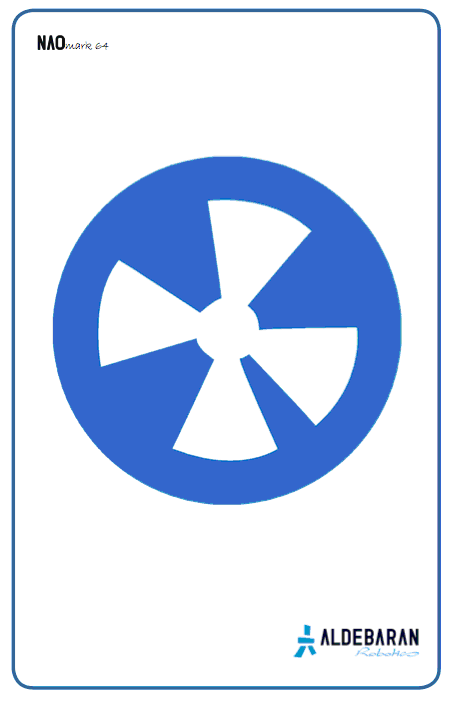
\includegraphics[width=0.3\textwidth, angle=0]{img/nao_7.png}
    \caption{Beispiel für einen NAOMarker mit ID 64.}
    \label{nao_marker}
\end{figure}

\subsection{Marker Konstruktion für NXT}
Da, wie bereits beschrieben, die NAOMarker mit der Erkennung von NXT-Robotern einher geht, haben wir uns Gedanken gemacht, wie ein oder mehrere Marker auf den “Erkundungsroboter” platziert werden können, um diese an möglichst jedem Punkt auf dem unbekannten Feld zu lokalisieren. Wir haben uns dafür entschieden sechs verschiedene Marker pro NXT zu verwenden, was von oben betrachtet einem gleichseitigen Hexagon entspricht. Auf den Bildern X und Y kann man diese noch einmal genauer sehen. Dadurch, dass wir von jeder Seite des NXTs eine andere ID erkennen, die einen NAOMarker codiert, können wir auf 60° genau die Drehung des NXTs unterscheiden. Dies wird unterteilt in 0° bzw. 360° (front), 60° (rechts vorn), 120° (rechts hinten), 180° (hinten), 240° (links hinten), 300° (links vorn). Daraus ergibt sich ein Vorteil: Bei unseren Tests haben wir festgestellt, dass sobald sich die Konstruktion in erkennbarer Reichweite für den NAO befindet, die Marker immer erkannt werden können, egal in welchem Winkel die Konstruktion zum NAO steht. D.h. ein Marker wird auch dann erkannt, wenn er im schlechtesten Fall in einem Winkel von 30° zur Kamera steht.

\begin{figure}[ht]
    \centering
  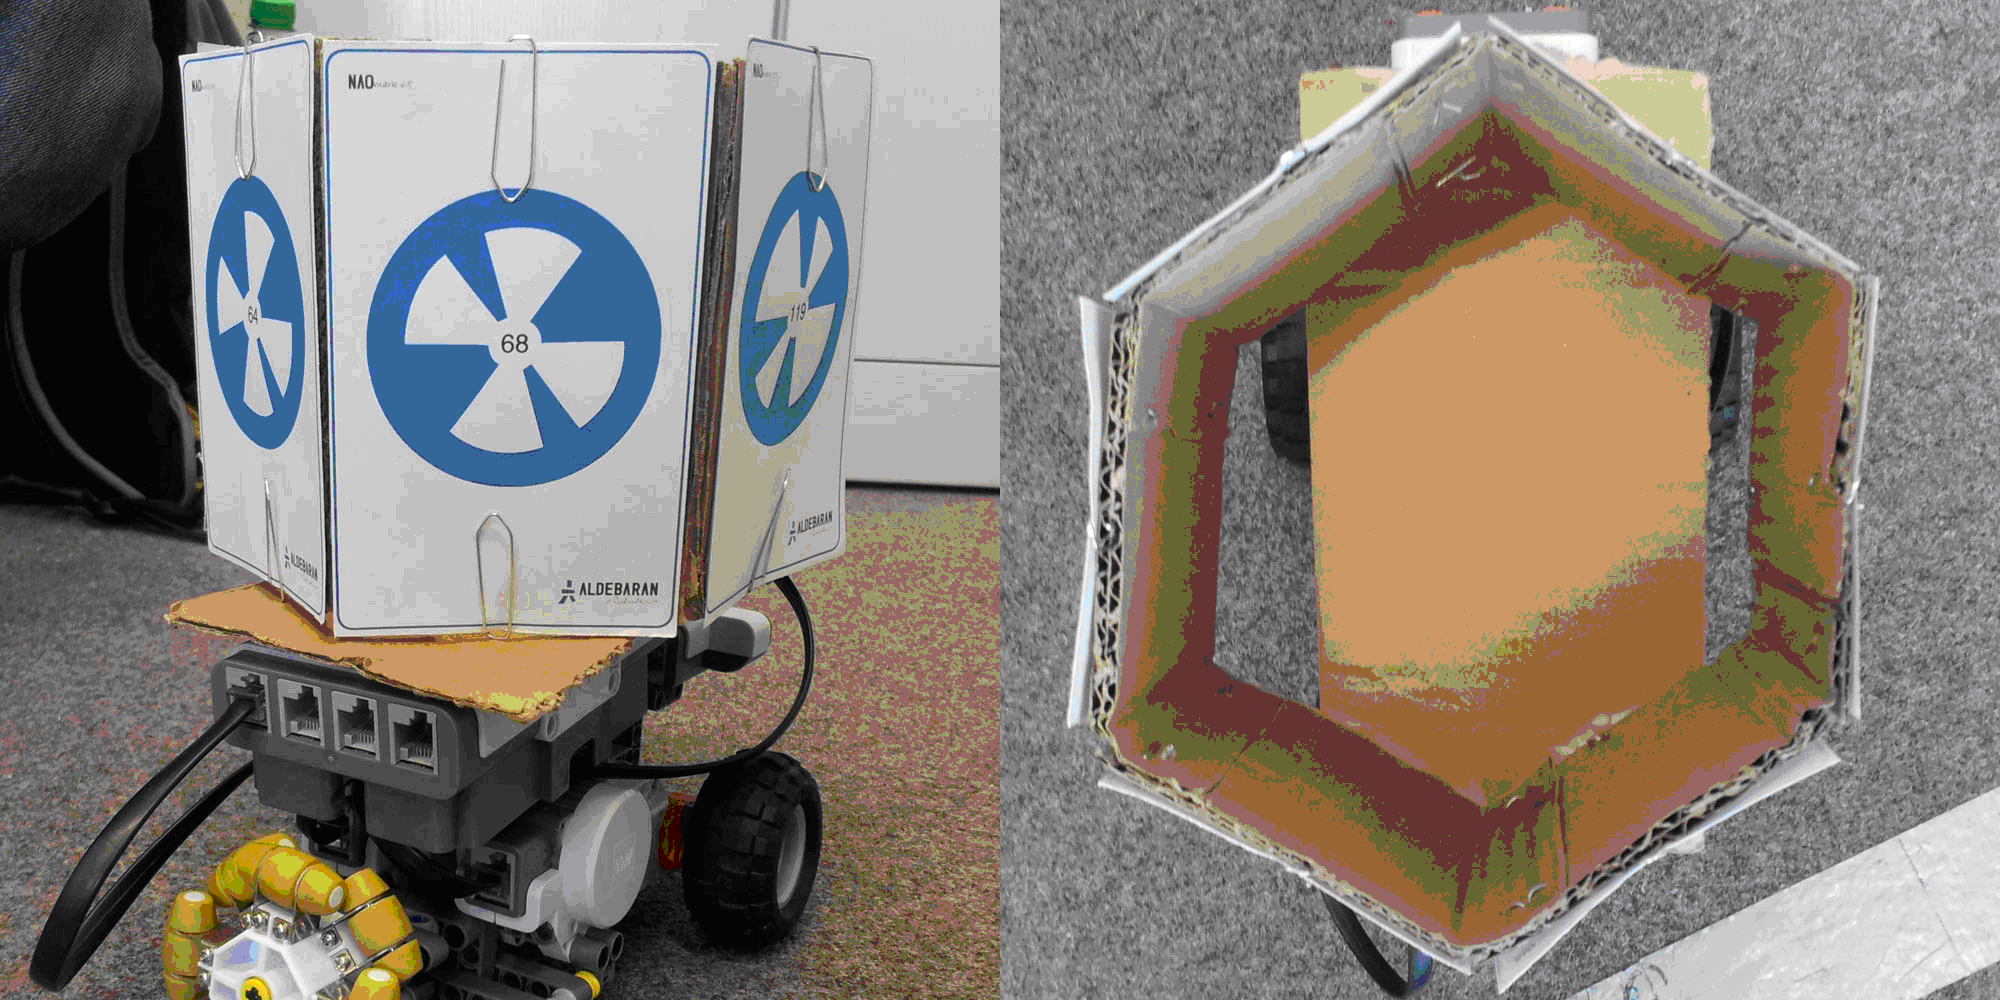
\includegraphics[width=0.9\textwidth, angle=0]{img/nao_8.png}
    \caption{Markerkonstruktion für NXT Roboter}
    \label{nao_marker2}
\end{figure}

Da wir unser Konstruktion auf einen relativ kleinen NXT platzieren und Einsparungen in der Größe der Marker machen wollten, haben wir den Kreis mit Struktur ausgeschnitten und auf den NXT platziert. Bei späteren Tests mit den ausgeschnittenen Markern haben wir allerdings herausgefunden, dass eine richtige Erkennung nur dann möglich ist, wenn er die auf dem Bild X die erkennbare Umrandung beibehält. Die Marker, die wir benutzen, sind wegen Platzgründen nur halb so Groß und im Durchmesser ca. 6 cm. Trotz kleinerer NAOMarker werden diese auch noch bei bis zu  160 cm erkannt. Man sollte außderdem wissen, dass die Erkennung der NAOMarker nur dann funktioniert, wenn die Marker wie in den Abbildungen im Hochformat vorliegt. Die Farbe ist allerdings egal nur die Struktur und der beschrieben Rand sind dagegen essentiell.
Da wir in unserem Szenario von drei NXTs ausgehen, die das Gelände erkunden und kalibriert werden müssen, bräuchten wir 18 Marker. Weil allerdings, wie bereits erwähnt, nur die 10 Marker vorhanden waren, haben wir uns dazu entschieden farbige Marker für die Unterscheidung zwischen den NXTs zu benutzen. Dies wird im Abschnitt X Farberkennung beschrieben.

\subsection{Auslesen der übergebenen Werte}
Die Markerinformationen können m.H. dieses Python Programmcodes abgegriffen werden: 
markerInfo = ALProxy(``ALMemory'', self.IP, self.PORT).getData``LandmarkDetected'')
\\
Die Daten in Form eines Arrays bei der Marker Detektion können wie folgt interpretiert werden: 
markerInfo = [[Zeitstempel\_in\_s, Zeitstempel\_in\_ms], [Markerarray\_0, Markerarray\_1, .. , Markerarray\_N], [MarkerInfoArray\_a], [MarkerInfoArray\_b]], Kamerainfo]
N ist die Anzahl der erkannten Marker. Je mehr der NAO an Marker erkennt, desto größer wird das Array mit den bereitgestellten Informationen. 
\\
Markerarray\_i, in der sich die spezifischen Daten für die Größe und Winkel der einzelnen Marker befindet, ist wie folgt aufgebaut:
Markerarray\_i = [[Form, Alpha, Beta, GroesseX, GroesseY, Titel], [MarkerID]].
MarkerInfoArray\_a und b sind jeweils sechs unbekannte Werte und auch bei Aldebaran nicht weiter kommentiert oder erklärt.
Was die Angaben für Form (shape) und Titel (heading) bedeuten, ist gänzlich unbekannt und die Dokumentation von Aldebaran gibt hier auch keine Informationen. Die Angabe zur Größe des erkannten Markers für X und Y sind zueinander immer gleich (abhängig von der Entfernung des Markers).
Die interessanten und für uns wichtigen Werte sind in Alpha und Beta gespeichert. Alpha gibt die Ausrichtung der Kamera nach rechts und links an, also den yaw-Winkel und Beta ist die Ausrichtung für oben und unten, also der pitch-Winkel. Alpha liegt in [-0.3, 0.3], wobei negative Werte rechts und positive Werte links vom Mittelpunkt des Kamerabildes liegen. Beta liegt  in [-0.25, 0.1], wobei negative Werte für oben und positive Werte für unten zu interpretieren sind.

\subsection{Farberkennung}
Da es von Aldebaran nur 10 frei verfügbare NAOMarker gibt, aber wir insgesamt 18 Marker brauchen, haben wir uns dafür entschieden jedem NXT die gleichen Marker mit unterschiedlichen Farben zuzuteilen. Dadurch ist es uns möglich über die Farbe den NXT zuzuordnen und über den Marker selbst die Ausrichtung des NXTs herauszufinden.
Die Triangulation ruft die Farberkennung auf, sobald ein Marker gefunden und auf ihn zentriert worden ist, der einem einem NXT zugeordnet werden soll. Die Farberkennung gibt dann die Farbe des zentrierten Markers zurück.
Zur Bildverarbeitung greifen wir auf OpenCV zu, das schon auf dem NAO installiert ist und viele vorgefertigte Methoden zum Verarbeiten bereitstellt.
\\
Zuerst nimmt die NAO Kamera ein Foto auf und speichert dies auf dem NAO. Zusätzlich wird der Pixelarray von dem Foto gespeichert, aus dem mit der Python Image Library ein Bild erzeugt wird. 
Danach wird anhand der gemessenen Markergröße ein Rechteck aus dem Bild ausgeschnitten, in dem sich der Marker befindet. Das Bild wird dann zu HSV(Hue, Saturation, Value) konvertiert, um leichter die Farbe bestimmen zu können.
Nun wird das Bild für jede Farbe nacheinander auf einen bestimmten HSV Bereich begrenzt bzw die Pixel in dem restlichen Bereich ausgeblendet. Um das Rauschen in den Fotos nicht zu berücksichtigen, wird ein Mindestbereich an Pixeln gewählt. Zusätzlich wird mit dem Pythagoras der Abstand des Bereichs zum Bildmittelpunkt berechnet. Im letzten Schritt werden die Bereiche von jeder Farbe miteinander verglichen und die Farbe mit dem Bereich, welche den kürzesten Abstand zum Mittelpunkt hat, als die wahrscheinlichste Farbe zurückgegeben. Falls keine der vorhandenen Farben gefunden wurde, dann wird dies zurückgegeben.


\subsection{Triangulation}
Die Idee zur Abstandsberechung durch Triangulation kam uns durch die Arbeit von [Stepan Krivanec et. al. 2009]\footnote{ftp://cmp.felk.cvut.cz/pub/cvl/articles/prusa/Krivanec-TR-2010-21.pdf}. In der Quelle wird beschrieben, dass eine Abstandsberechnung mit Hilfe der NAOMarker nur mit zwei NAOs möglich ist oder bei Bewegen des NAOs an eine andere Position, da der Roboter keine Stereo Kamera besitzen. Tatsächlich aber kann man auch über nur einen NAO triangulieren. Die Höhe der NAO-Kamera (obere Kamera) lässt sich einfach ausmessen und ist in der Initialpostition, wenn der NAO steht, genau 50 cm vom Boden entfernt. Außerdem werden, wenn ein NAOMarker erkannt wird, u.a. zwei Winkel zurückgegeben, die die horizontalen und vertikalen Winkel angeben, in dem sich die NAO Kamera zum Marker befindet.

\begin{figure}[ht]
    \centering
  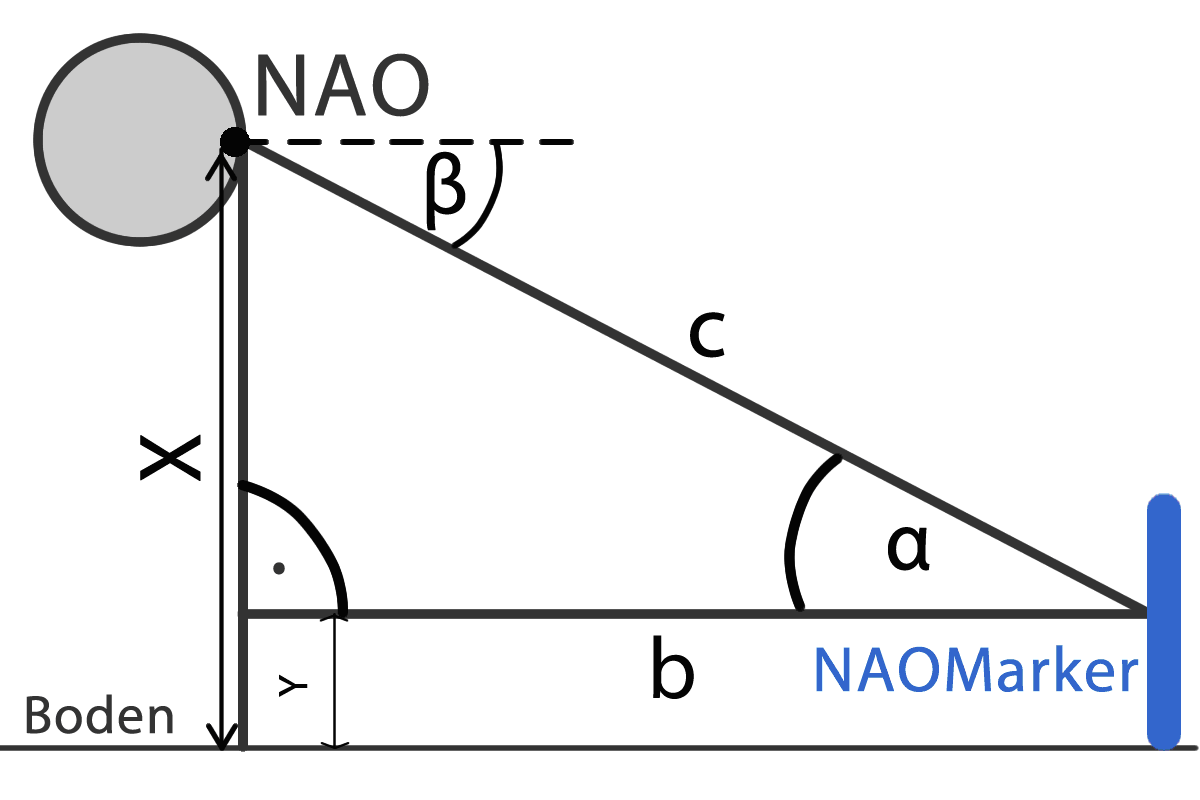
\includegraphics[width=0.5\textwidth, angle=0]{img/nao_9.png}
    \caption{Darstellung des Aufbaus zur Markerdetektion}
    \label{nao_marker3}
\end{figure}

Mit Hilfe der Höhe und des Winkels kann nun Gleichung die Entfernungsberechnung erfolgen. Dazu verwenden wir die einfache trigonometrische Funktion   .
Die angepasste trigonometrische Funktion lautet:  . Der Winkel  kann aus dem bereits beschriebenen Markerarray\_i als Alpha extrahiert werden. 
Durch Umstellung erhalten wir den gesuchten Abstand mit  . Man beachte, dass in die Berechnung auch die Höhe des Markermittelpunktes Y eingeht und vorher genau ausgemessen werden sollte.

\section{NAOWalk mit RedBall Tracking}

Wie schon im Punkt ``4.3 NAOWalk'' beschrieben, ist der NAO nicht im Stande selbst kurze Strecken exakt zu laufen. Daher wäre es nicht möglich den NAO sich selbst über die Karte navigieren zu lassen. 
Um den NAO dennoch zum Ziel zu navigieren, ist es nötig Fixpunkte im Gelände zu haben, an denen er sich orientieren und seine Laufbahn korrigieren kann.
Realisiert werden diese Fixpunkte über einen roten Ball, den der NAO visuell erkennen und verarbeiten kann. Dieser ist auf einem der NXT's befestigt.
\\
Der Vorgang der Wegfindung basiert nun auf einem Pfad, den das MCC aus der Karte berechnet. Für diesen Vorgang verweise ich auf den Punkt Pfadberechnung in der MCC-Dokumentation.
Letztendlich entsteht dabei ein Pfad, der in Teilabschnitte unterteilt ist, die jeweils nur durch gerade Strecken miteinander verbunden sind.
\\
Entlang dieses Pfades wird der NXT mit dem roten Ball auf die bestimmten Positionen geschickt und der NAO folgt ihm.
Um zu verhindern dass der NAO und NXT sich gegenseitig in die Quere kommen werden die einzelnen Abschnitte des Pfades noch wie folgt in Phasen aufgeteilt, wobei die Ausgangsbedingung ist, dass sich der NXT eine Position weiter auf dem Pfad befindet als der NAO:
\\
P0: Sofern kein Nxt mit rotem Ball in Sicht ist, versuche einen zu finden
P1: NAO läuft gerade bis auf einige cm Abstand auf den NXT zu
P2: NAO speichert die Position des NXT
P3: NAO meldet dem MCC vor dem NXT angekommen zu sein
P4: MCC gibt NXT den Befehl, auf die nächste Position zu fahren
P5: NAO läuft auf die gespeicherte Position und richtet sich neu nach dem NXT aus
\\
Nach diesem Ablauf werden alle Teilabschnitte des Pfades abgearbeitet, bis der NAO sich im Zielgebiet befindet.
\\
Im Folgenden werden die einzelnen Fähigkeiten erklärt, die der NAO mitbringen muss, um oben genannte Phasen erfolgreich abschließen zu können.
\\
\\
\subsection*{P0:}
Der NAO muss entscheiden können, ob er einen roten Ball sieht oder nicht. Hierbei wird das NAOQi API Modul ALRedBallTracker benutzt, welche an das Event  redBallDetected() der ALRedBallDetection des ALVision-Moduls gekoppelt ist. ALRedBallTracker bietet die Funktion isNewData() an, welche true zurückgibt falls ein neuer roter Ball seit der letzten Abfrage erkannt worden ist. Um zu entscheiden, ob ein Ball erkannt wird, benutzt die Methode hasBall() der NAOWalk-Klasse diese Funktionalität.
\\
Liefert hasBall() false, so scannt er sein Blickfeld, indem er methodisch seinen Kopf derart bewegt, dass das maximal mögliche Sichtfeld abgedeckt wurde. Hat er danach noch immer nichts gefunden, dreht er sich um seine senkrechte Körperachse um 90 Grad und wiederholt den Vorgang bis er sich vollständig um die eigene Achse gedreht hat. Findet er letztendlich einen Ball, so richtet er sich nach diesem mit der privaten Methode \_\_turnToBall() aus. Diese Funktionalität bietet die retrieveBall()-Methode aus der NAOWalk-Klasse.
\\
\\
\subsection*{P1:}
Zusätzlich zu der Grundfunktionalität des Laufens in eine gegeben Richtung, welche über das ALMotion-Modul mittels der Methode walkTo()  gegeben wird, muss der NAO hierbei seine Laufbahn stetig korrigieren können. Da walkTo() dies per se nicht ermöglicht, muss eine Abweichung von der Laufbahn festgestellt werden können. Dies wird über eine Abfrage des Drehwinkels des Kopfgelenks realisiert. Die visuelle Erkennung des roten Balls ermöglicht es dem NAO, diesen permanent in der Mitte seines Sichtfeldes zu halten. Hierbei wird nur der Kopf bewegt. Bewegt sich der NAO relativ zum Ball, neigt bzw. dreht er den Kopf. Ab einer bestimmten Abweichung des Drehwinkels zum Nullpunkt ist davon auszugehen, dass der NAO seine gerade Bahn zum NXT verlassen hat und er wird gestoppt, richtet sich neu nach dem NXT mit turnToBall() aus und läuft erneut los.
\\
Da der Sichtbereich der oberen Kamera des NAO's bei aufgerichtetem Körper zu weit von ihm entfernt endet, um nah genug an den NXT heran zu kommen ohne ihn aus dem Blick zu verlieren, muss während der Annäherung ab einer bestimmten Distanz auf die untere Kamera umgeschaltet werden. Ein Beugen des Oberkörpers zu diesem Zweck führt zu einer erheblichen Instabilität der gesamten Laufanimation, sodass ein Hinfallen des Roboters unausweichlich ist. Dies geschieht über die beiden privaten Methoden \_\_setTopCamera() und \_\_setBottomCamera() der NAOWalk-Klasse.
\\
Zur Berechnung der Distanz wird die Methode getPosition() von ALRedBallTracker benutzt. 
Hierzu muss noch der SPACE\_TORSO eingeführt werden: 
NAO kennt verschiedene karthesische Räume, wie zum Bsp. SPACE\_TORSO, bei welchem ein 3D-Koordinatensystem in die Körpermitte des NAO gelegt wird. 
getPosition() liefert [x,y,z]-Koordinaten des Balls in SPACE\_TORSO zurück, wobei x die Distanz nach vorne bzw hinten, y nach rechts bzw links und z die Höhe ist. 
\\
Um festzustellen, ob die Rückgabewerte von getPosition() für eine automatisierte  Verarbeitung geeignet sind, wurde eine Testreihe angelegt, deren Ergebnis dem Diagramm unten zu entnehmen ist. Real bezeichne dabei die in der realen Welt gemessenen Werte.

\begin{figure}[ht]
    \centering
  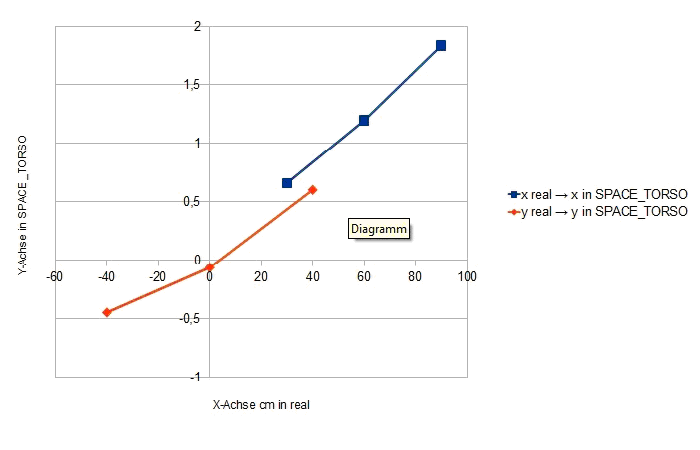
\includegraphics[width=0.9\textwidth, angle=0]{img/nao_10.png}
\end{figure}

Es ist deutlich zu sehen, dass der Werteverlauf bei x sowie y linear ist. z kann hierbei ignoriert werden, da es für die Berechnung des Abstandes irrelevant ist. Die geringen Abweichungen  ergeben sich aus Messungenauigkeiten. 
Daraus folgt, dass die cm in SPACE\_TORSO sich aus den Rückgabewerten mittels einer linearen Funktion in cm in real interpolieren lassen. 
Ergo ipso facto lassen sich exakte Werte zur Weiterverarbeitung gewinnen.
\\
Da die Höhe des Balls konstant bleibt, lässt sich der Abstand aus der Auslenkung der x- und y-Achse interpolieren. Dies geschieht mit einem simplen Pythagoras und ist in die private Methode \_\_getDistance() ausgelagert.
Diese gesamte Funktionalität ist in der walkUpToBall()-Methode aus der NAOWalk-Klasse implementiert.
\\
\\
\subsection*{P2:}
Um die Position eines NXT zu speichern legt der NAO ein Datenfeld mit den Koordinaten der getPosition()-Methode zum Zeitpunkt der Speicherung mittels \_\_safePosition() an. Nun kann er diese Daten benutzen, wenn sich der NXT schon auf die nächste Position bewegt hat.
\\
\\
\subsection*{P5:}
Aus der vorher gespeicherten Position relativ zum NAO in SPACE\_TORSO, kann der NAO nun interpolieren, wie weit er sich bewegen muss um exakt auf dieser Position zu stehen. Dies geschieht in der walkToPosition()-Methode der NAOWalk-Klasse. Dieser Abstand ist sehr kurz und kann daher ohne korrektur vom NAO gelaufen werden.
Sollte sich der NAO noch nicht im Zielgebiet befinden, richtet er sich mit retrieveBall() erneut nach dem NXT mit dem roten Ball aus und der Phasendurchlauf beginnt von vorne.

\section{Probleme \& Lösungen}

\subsection{NAO}
Am Anfang haben wir uns immer direkt mit einem LAN Kabel zu dem NAO verbunden, wobei diese Verbindung sehr störanfällig war. 
Die Konnektivität erfolgte später über WLAN. Dies war sehr viel stabiler und störunanfälliger, jedoch kam es häufig trotzdem zu Verbindungsproblemen, die meistens mit einem Neustart des NAO behoben werden konnten.
Die Sensoren des NAO waren bei uns teilweise sehr anfällig und ungenau.
Wenn der NAO längere Zeit mit Stiffness stand, dann haben sich die Motoren so stark erhitzt, dass der NAO erst abkühlen musste bevor er weiter verwendet werden konnte.
Teilweise ist auch das NAOqi grundlos abgestürzt und der NAO ist daraufhin einfach hingefallen.

\subsection{NAOMarker}
Der NAO sollte eigentlich maximal 6 Marker gleichzeitig erkennen, jedoch hat er bei uns auch mehr Marker gleichzeitig erkannt. Die Markererkennung arbeit auf einem bestimmten Bereich vor dem NAO, ca. zwischen 20 cm und 140 cm, akkurat. Wenn der Marker jedoch näher oder weiter entfernt ist, dann erkennt der NAO den Marker entweder überhaupt nicht oder verwechselt ihn mit einem anderen Marker.

\subsection{Triangulation}
Die Triangulation schwankt durch die Ungenauigkeit der Markererkennung, wodurch die Abweichung bis zu 10 cm betragen kann.

\subsection{Farberkennung}
Die Bilder der Kamera sind durch die verschiedenen Beleuchtungsverhältnisse sehr unterschiedlich von der Helligkeit und dem Kontrast. Am Anfang haben wir Versuche mit der Farbe gelb und später schwarz durchgeführt, jedoch war gelb immer zu schwer von weiß und schwarz zu schwer vom Untergrund zu unterscheiden und deshalb sind diese weggefallen. Bei den anderen Farben haben wir es nach vielen Feinjustierungen geschafft, die unterschiedlichen Farben über verschiedene Distanzen zu erkennen.
Durch die Zentrierung der Kamera NAO auf die einzelnen Marker wurde auch das Problem der verschiedenen Farbbereiche im Sichtfeld, wobei nicht nach der Größe der Farbbereiche beurteilt werden darf, gelöst.
Die Farberkennung dauerte am Anfang auch sehr lange, aber konnte durch die Wahl des Bildtyps von JPG anstatt PNG stark beschleunigt werden.\\